\PassOptionsToPackage{unicode=true}{hyperref} % options for packages loaded elsewhere
\PassOptionsToPackage{hyphens}{url}

\documentclass[ignorenonframetext,]{beamer}
\usepackage{longtable,booktabs} % for longer tables
\usepackage{pgfpages}
\setbeamertemplate{caption}[numbered]
\setbeamertemplate{caption label separator}{: }
\setbeamercolor{caption name}{fg=normal text.fg}
%\beamertemplatenavigationsymbolsempty
% Prevent slide breaks in the middle of a paragraph:
\widowpenalties 1 10000
\raggedbottom
\setbeamertemplate{part page}{
\centering
\begin{beamercolorbox}[sep=16pt,center]{part title}
  \usebeamerfont{part title}\insertpart\par
\end{beamercolorbox}
}
\setbeamertemplate{section page}{
\centering
\begin{beamercolorbox}[sep=12pt,center]{part title}
  \usebeamerfont{section title}\insertsection\par
\end{beamercolorbox}
}
\setbeamertemplate{subsection page}{
\centering
\begin{beamercolorbox}[sep=8pt,center]{part title}
  \usebeamerfont{subsection title}\insertsubsection\par
\end{beamercolorbox}
}
\AtBeginPart{
  \frame{\partpage}
}
\AtBeginSection{
  \ifbibliography
  \else
    \frame{\sectionpage}
  \fi
}
\AtBeginSubsection{
  \frame{\subsectionpage}
}
\usepackage{lmodern}
\usepackage{amssymb,amsmath}
\usepackage{ifxetex,ifluatex}
%\usepackage{fixltx2e} % provides \textsubscript
\ifnum 0\ifxetex 1\fi\ifluatex 1\fi=0 % if pdftex
  \usepackage[T1]{fontenc}
  \usepackage[utf8]{inputenc}
  \usepackage{textcomp} % provides euro and other symbols
\else % if luatex or xelatex
  \usepackage{unicode-math}
  \defaultfontfeatures{Ligatures=TeX,Scale=MatchLowercase}
\fi
\usecolortheme{seagull}
% use upquote if available, for straight quotes in verbatim environments
\IfFileExists{upquote.sty}{\usepackage{upquote}}{}
% use microtype if available
\IfFileExists{microtype.sty}{%
\usepackage[]{microtype}
\UseMicrotypeSet[protrusion]{basicmath} % disable protrusion for tt fonts
}{}
\IfFileExists{parskip.sty}{%
\usepackage{parskip}
}{% else
\setlength{\parindent}{0pt}
\setlength{\parskip}{6pt plus 2pt minus 1pt}
}
\usepackage{hyperref}
\hypersetup{
            pdfborder={0 0 0},
            breaklinks=true,
            colorlinks = true,
            linkcolor = blue, 
            urlcolor = blue}
\urlstyle{same}  % don't use monospace font for urls
\usepackage{ragged2e} % horiazontal alignment
\newif\ifbibliography
\setlength{\emergencystretch}{3em}  % prevent overfull lines
\providecommand{\tightlist}{%
  \setlength{\itemsep}{0pt}\setlength{\parskip}{0pt}}
\setcounter{secnumdepth}{0}
% set default figure placement to htbp
\makeatletter
\def\fps@figure{htbp}
\makeatother

\definecolor{yaleblue}{rgb}{0.06, 0.3, 0.57}
\definecolor{airforceblue}{rgb}{0.36, 0.54, 0.66}
\definecolor{blue(ncs)}{rgb}{0.0,0.53, 0.74}
\definecolor{bluegray}{rgb}{0.4, 0.6, 0.8}
\definecolor{cerulean}{rgb}{0.0,0.48, 0.65}
\definecolor{darkgreen}{rgb}{.2,.5,.6}
\definecolor{grey}{rgb}{.38,.38,.38}
\definecolor{chromeyellow}{rgb}{1.0, 0.65, 0.0}
\definecolor{darkblue}{rgb}{0, .25, .53}
\definecolor{darkorange}{rgb}{1, .27, 0}
\usepackage{setspace} 
\usepackage{caption}
\captionsetup[figure]{labelformat=empty}
%rainbow colors
\definecolor{red}{rgb}{.89,.01,.01}
\definecolor{orange}{rgb}{1,.55,0}
\definecolor{yellow}{rgb}{1,.93,0}
\definecolor{green}{rgb}{0,.5,.15}
\definecolor{indigo}{rgb}{0,.3,1}
\definecolor{violet}{rgb}{.45,.16,.51}
\definecolor{lightblue}{rgb}{0,.5,1}

\setbeamercovered{transparent}
\setbeamertemplate{footline}[frame number] %add frame numbers


\newcommand\mytext{\color{grey}{Anne Lochner \& Nicole Cruz}}
\makeatother
\setbeamertemplate{footline}
{%
  \leavevmode%
  \hbox{\begin{beamercolorbox}[wd=.5\paperwidth,ht=2.5ex,dp=1.125ex,leftskip=.3cm,rightskip=.3cm]{author in head/foot}%
  \mytext
  \end{beamercolorbox}%
  \begin{beamercolorbox}[wd=.5\paperwidth,ht=2.5ex,dp=1.125ex,leftskip=.3cm,rightskip=.3cm plus1fil]{author in head/foot}%
    \usebeamerfont{author in head/foot}\insertshortauthor \hfill\insertframenumber
  \end{beamercolorbox}}%
  \vskip0pt%
}
\makeatletter


\title{\color{yaleblue}\\ Multilevel modelling}
\vspace{-.8cm}

\author[\color{grey}{Computational Linguistics Meeting 2026}]{
\color{grey} \\ \footnotesize{  \vspace{.2cm}  
 \vspace{-.5cm}  
 \href{https://art.djnavarro.net/gallery/tiling/}{
 
\includegraphics[width=5cm]{graphs/navarro_tiling}
 \vspace{-.25cm}  
 }}} 
    
\date{\footnotesize{ \footnotesize{Anne Lochner \& Nicole Cruz \\
 \color{teal}
 \vspace{1 mm} 
 Computational Linguistics Meeting 2026  \\ 
 \vspace{1 mm} 
\scriptsize{\color{grey}{Utrecht, 2. December 2026}
}}}}


\begin{document}

%
\begin{frame}[plain] %suppress frame number
\titlepage
\end{frame}
%\frame{\titlepage}

%
\begin{frame}{\color{darkblue}Contents}
  \vspace{2.2cm}
    \tableofcontents
     \vspace{2.8cm}
     
\end{frame}


%%%%%%%%%%%%%%%%%%%%%%%%%%%%%%%%%%%%%%%%%
\section{\(\color{teal}\textrm{Introduction: Why multilevel?}\)}



%
\begin{frame}{\color{darkblue}Multilevel}

\begin{itemize}
\tightlist 
\item Multilevel resp. hierarchical models allow data analysis at several levels of aggregation.  
\pause
\item E.g. level 1:  single data points of a student, level 2: student, level 3: school, level 4: city, level 5: country...
\pause
\item The levels are numbered from bottom to top, and from specific to general. 
\pause
\item Parameter estimates are drawn from nested distributions.
\end{itemize}

\end{frame}


%
\begin{frame}{\color{darkblue}Mixed}

\begin{itemize}
\tightlist 
\item Multilevel models are sometimes called mixed, because they allow the analysis not only of means but also of variances.
\pause
\begin{itemize}
\tightlist 
\item[-] Parameters for means: "{\color{teal}{fixed effects}}"
\item[-] Parameters for variances: "{\color{teal}{random effects}}"
\end{itemize}
\end{itemize}

\end{frame}

%
\begin{frame}{\color{darkblue}Multilevel data structures}

\begin{itemize}
\tightlist 
\item Generalization of simple linear regression and ANOVA to complexer data with nested groups.
\pause
\item When hierarchical data is analysed only at one level, this can lead to under- or overestimation of effects, which undermines the interpretability of the findings. 
\pause
\begin{itemize}
\tightlist
\item[$\rightarrow$] Ecological and atomistic fallacy, Simpson's paradox 
\end{itemize}
\end{itemize}
\end{frame}

%
\begin{frame}{\color{darkblue}Ecological fallacy}

\begin{block}{}
An ecological fallacy is a fallacy in the interpretation of statistical data. It occurs when a data pattern that was observed at the group level (e.g. the group mean) is generalised to the level of individual data points. This is a fallacy because the pattern at one level of aggregation does not necessarily coincide with the pattern at another level of aggregation. 
\end{block}
\pause
Ecological fallacy in which the direction of an effect switches between the group and the individual levels: {\color{teal}{Simpson's Paradox}}.

\par\begin{spacing}{.5}\begingroup\tiny(\href{https://www.semanticscholar.org/paper/Statistik-und-Forschungsmethoden-Eid-Gollwitzer/6ea32c37f2621c9267f1c28ba2eaf7c7b29d4710}{Eid et al., 2010}; \href{https://doi.org/10.2307/2087176}{Robinson, 1950}).\endgroup\end{spacing}


\end{frame}

%
\begin{frame}{\color{darkblue}Ecological fallacy: example}

\begin{figure}
\centering
\href{https://en.wikipedia.org/wiki/Ecological_fallacy}{
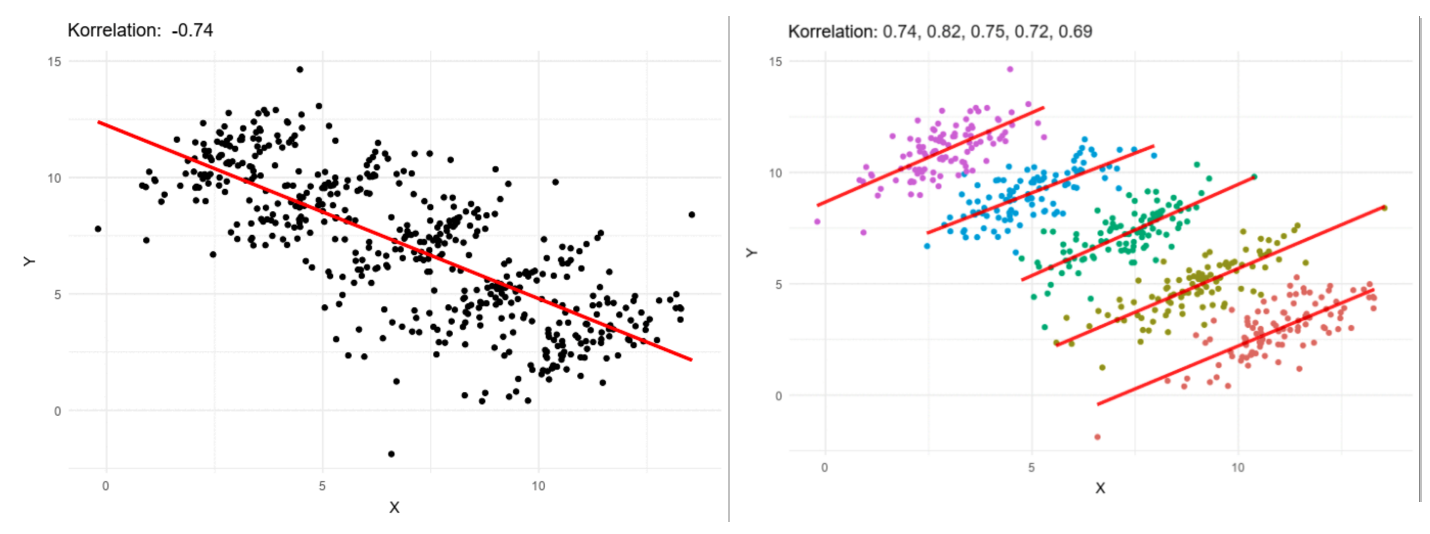
\includegraphics[width=.6\textwidth]{graphs/simpson2}}
\end{figure}

\small{{\color{teal}{\textit{A research team studies the relation between autonomy at the work place and work satisfaction. It conducts interviews in 5 companies, correlates autonomy with satisfaction and finds an overall negative correlation between the two. But the same correlation was positive in each individual company. They conclude that autonomy correlates positively with satisfaction in general, but that other variables such as income also influence satisfaction scores.}}}}

\par\begin{spacing}{.5}\begingroup\tiny(\href{https://www.semanticscholar.org/paper/Statistik-und-Forschungsmethoden-Eid-Gollwitzer/6ea32c37f2621c9267f1c28ba2eaf7c7b29d4710}{Eid et al., 2010, Ch. 19}).\endgroup\end{spacing}

\end{frame}

%
\begin{frame}{\color{darkblue}Heteroscedasticity}

\begin{itemize}
\tightlist
\item Hierarchical data violate the assumption of homoscedasticity (i.e. variance homogeneity) from linear regression. 
\pause
\item Variance within groups tends to be smaller than variance between groups. (e.g. learning environment of students in the same class is more similar than of students in different classes). 
\pause
\item In multilevel analyses this is no problem. On the contrary: differences between variances can themselves become the subject of new research hypotheses.
\end{itemize}

\end{frame}

%
\begin{frame}{\color{darkblue}Advantages for theory development}


\begin{itemize}
\tightlist
\item Development of more differentiated, abstract theories.
\item Models in which one latent variable can be linked to several observations, and one observation to several latent variables (e.g. common-cause, common-effect networks).
\item Modelling measurement reliability and individual differences.
\end{itemize}

\par\begin{spacing}{.5}\begingroup\tiny (\href{https://doi.org/10.1016/j.jmp.2010.08.013}{Lee, 2011}; \href{https://link.springer.com/10.3758/s13428-023-02204-3}{Veenman et al., 2023}).\endgroup\end{spacing}

\end{frame}

%%%%%%%%%%%%%%%%%%%%%%%%%%%%%%%%%%%%%%%%%
\section{\(\color{teal}\textrm{Bias avoidance \& new hypotheses}\)}



%
\begin{frame}{\color{darkblue}Example questions for multilevel data}

\begin{figure}
\centering
\href{https://www.rdocumentation.org/packages/gapminder/versions/1.0.1}{
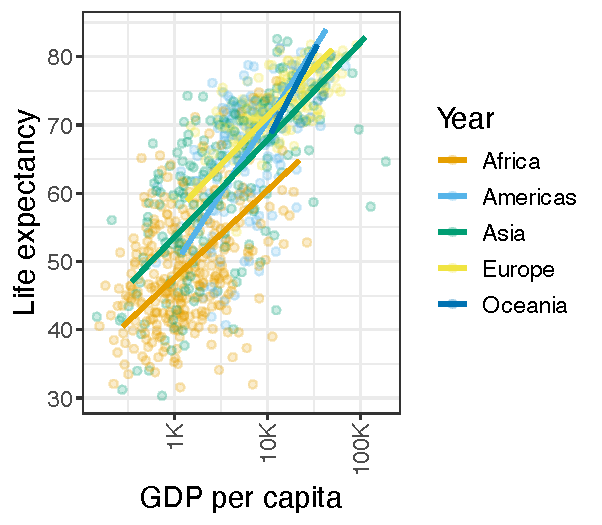
\includegraphics[width=.5\textwidth]{graphs/gapminder}}
\end{figure}

\vspace{-.5cm}

\pause
\small{
\begin{itemize}
\tightlist
\item[-] What is the overall intercept? 
\item[-] What is the overall regression slope? 
\item[-] Do the intercepts differ between groups? 
\item[-] Do the slopes differ between groups? 
\item[-] Are there cross-level interactions? 
\end{itemize}
}

\end{frame}

%
\begin{frame}{\color{darkblue}Example hypothesis about variance}

\begin{figure}
\centering
\href{https://www.worldhappiness.report}{
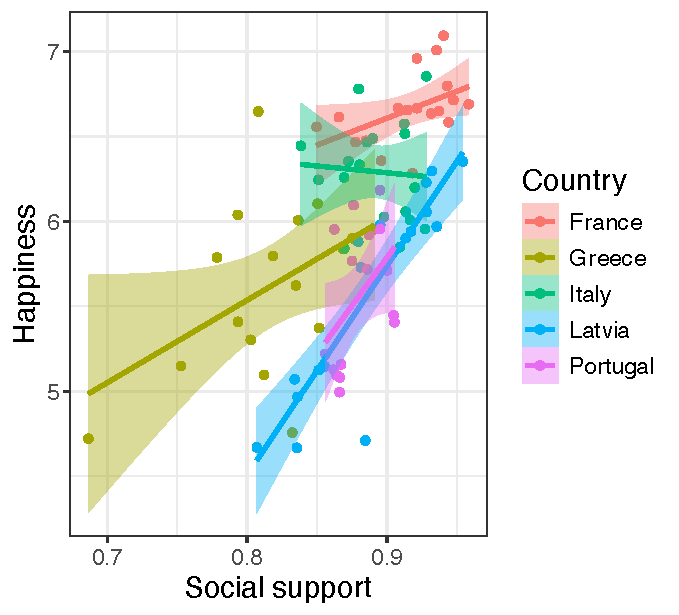
\includegraphics[width=.5\textwidth]{graphs/ghappysupport}}
\end{figure}

\pause
\begin{itemize}
\tightlist
\item For the data for the \href{https://www.worldhappiness.report/ed/2024/}{World Happiness Report 2024}: Is the variance in people's happiness smaller (or larger) for higher (or lower) values of social support?
\end{itemize}



\end{frame}


%
\begin{frame}{\color{darkblue}Two or more levels}

\begin{figure}
\href{https://www.taylorfrancis.com/chapters/edit/10.4324/9780429318405-2/introduction-mixed-models-experimental-psychology-henrik-singmann-david-kellen}
{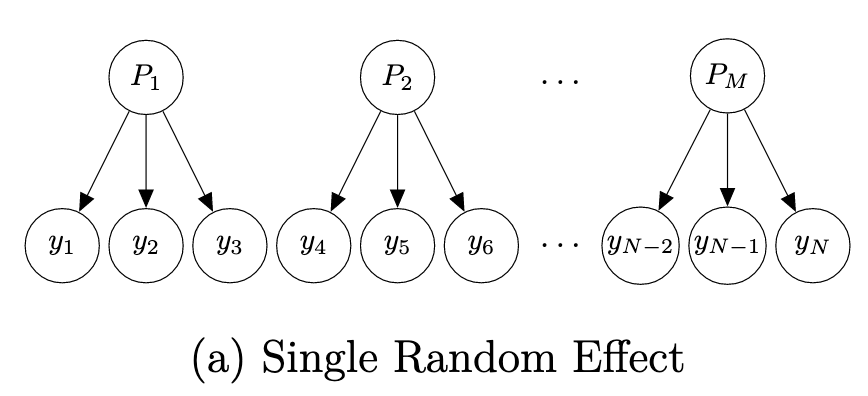
\includegraphics[width=.5\textwidth]{graphs/single_random}}
\end{figure}

\begin{columns}
\begin{column}{.5\textwidth}
\begin{figure}
\href{https://www.taylorfrancis.com/chapters/edit/10.4324/9780429318405-2/introduction-mixed-models-experimental-psychology-henrik-singmann-david-kellen}
{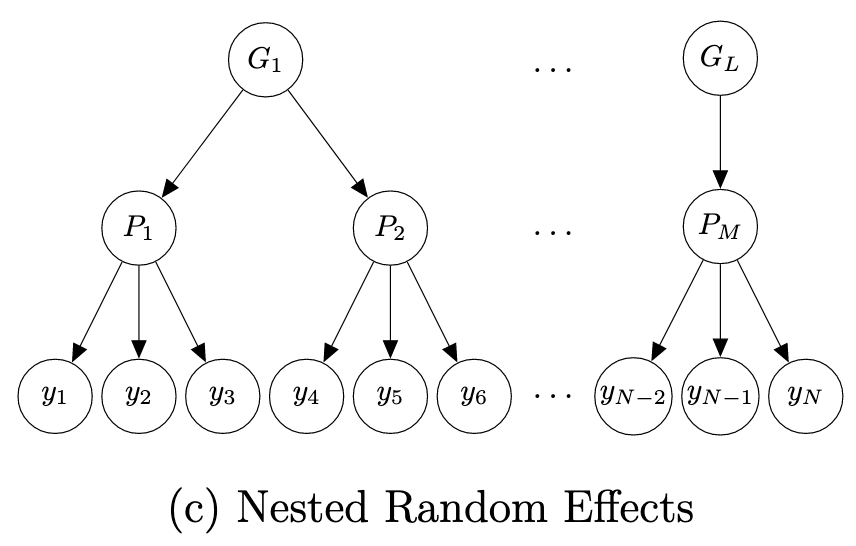
\includegraphics[width=.9\textwidth]{graphs/nested_random}}
\end{figure}
\end{column}
\begin{column}{.5\textwidth}
\begin{figure}
\href{https://www.taylorfrancis.com/chapters/edit/10.4324/9780429318405-2/introduction-mixed-models-experimental-psychology-henrik-singmann-david-kellen}
{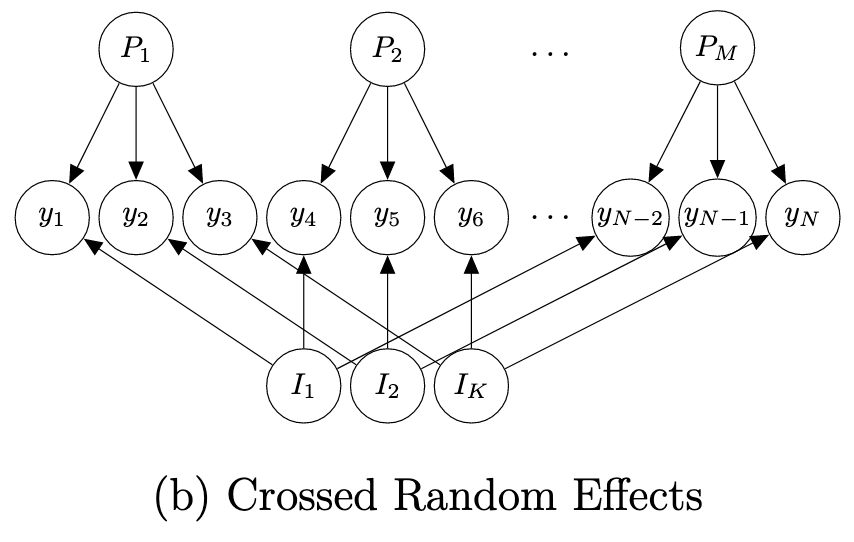
\includegraphics[width=.9\textwidth]{graphs/crossed_random}}
\end{figure}
\end{column}
\end{columns}

\end{frame}

%
\begin{frame}{\color{darkblue}Special case: within-participant designs}

\begin{figure}
\href{https://www.taylorfrancis.com/chapters/edit/10.4324/9780429318405-2/introduction-mixed-models-experimental-psychology-henrik-singmann-david-kellen}
{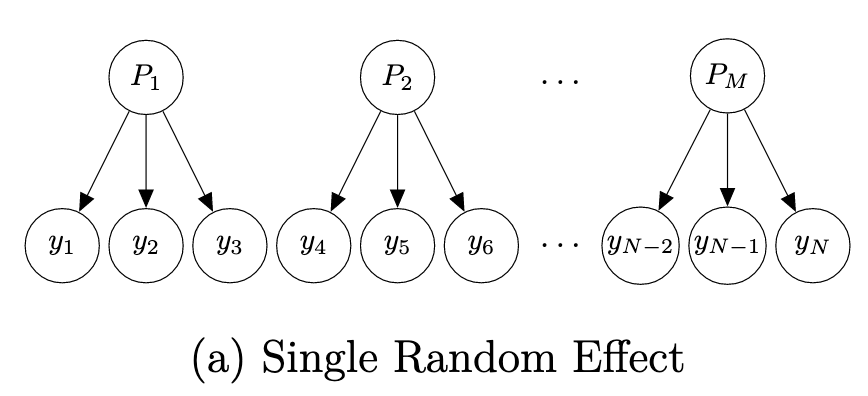
\includegraphics[width=.65\textwidth]{graphs/single_random}}
\end{figure}

\end{frame}


%
\begin{frame}{\color{darkblue}Which sample size?}

\begin{itemize}
\tightlist
\item Data analysed with multilevel models do not have a single sample size, but separate sample sizes at each level of aggregation (e.g. study with 20 trials per participant, 35 participants per school, 10 schools per country). 
\pause
\item These different sample sizes make it more difficult to determine degrees of freedom for statistical tests, and there is no single agreed on method for doing so.
\pause
\item This is less of a concern in the Bayesian framework, where posterior distributions can be estimated consistently regardless of the sample sizes involved.
\end{itemize}

\par\begin{spacing}{.5}\begingroup\tiny (\href{https://lme4.github.io/lme4/reference/pvalues.html}{Bates et al., 2026}).\endgroup\end{spacing}

\end{frame}

%
\begin{frame}{\color{darkblue}How many levels?}

Different criteria have been proposed for when to model an additional level of aggregation: 

\begin{itemize}
\tightlist
\item When there are 5 or more data points per cell in the design
\item When there are several measurements per individual (within participant design).
\item When individuals are in groups (e.g. classrooms in schools in districts; speakers in language traditions; plants in fields).
\item When we want to generalise beyond the specific individuals / experimental conditions measured.
\item When we want to estimate not only means but also variances. 
\item When the variance at the group level makes up a certain percentage (e.g. 10\% of the total sample variance).
\end{itemize}

\par\begin{spacing}{.5}\begingroup\tiny (\href{https://arxiv.org/abs/math/0504499}{Gelman, 2005}; \href{https://www.pearson.com/en-us/subject-catalog/p/using-multivariate-statistics/P200000003097/9780137526543}{Tabachnick \& Fidell, 2007}).\endgroup\end{spacing}

\end{frame}

%
\begin{frame}[t,fragile]{\color{darkblue}Interclass correlation}
\vspace{1 cm}

\begin{itemize}
\tightlist
\item The intraclass correlation ({\color{teal}{ICC}}) is the proportion of level 2 variance out of the total variance. 
\pause
\item For trials nested in individuals: proportion of the total variance attributable to interindividual differences.  
\end{itemize}
 {\color{teal}{\[ICC =  \frac{\sigma^2_{level2}}{\sigma^2_{level1} + \sigma^2_{level2}} \]}}

 \pause
 
 \vspace{-.2cm}
 Rule of thumb: open an aggregation level when ICC $\geq$ 10 \%.
 
\par\begin{spacing}{.5}\begingroup\tiny(\href{https://www.pearson.com/en-us/subject-catalog/p/using-multivariate-statistics/P200000003097/9780137526543}{Tabachnick \& Fidell, 2007}).\endgroup\end{spacing}

\end{frame}


%%%%%%%%%%%%%%%%%%%%%%%%%%%%%%%%%%%%%%%%%
\section{\(\color{teal}\textrm{Multilevel beyond regression}\)}

%
\begin{frame}{\color{darkblue}Causal Bayesian networks}

\begin{figure}
\centering
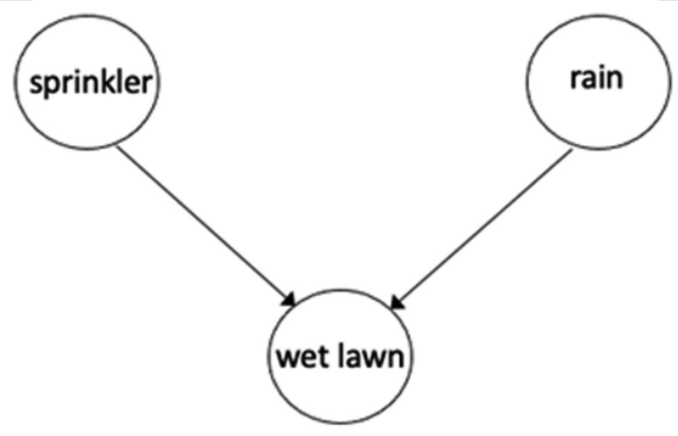
\includegraphics[width=.25\textwidth]{graphs/bn1}
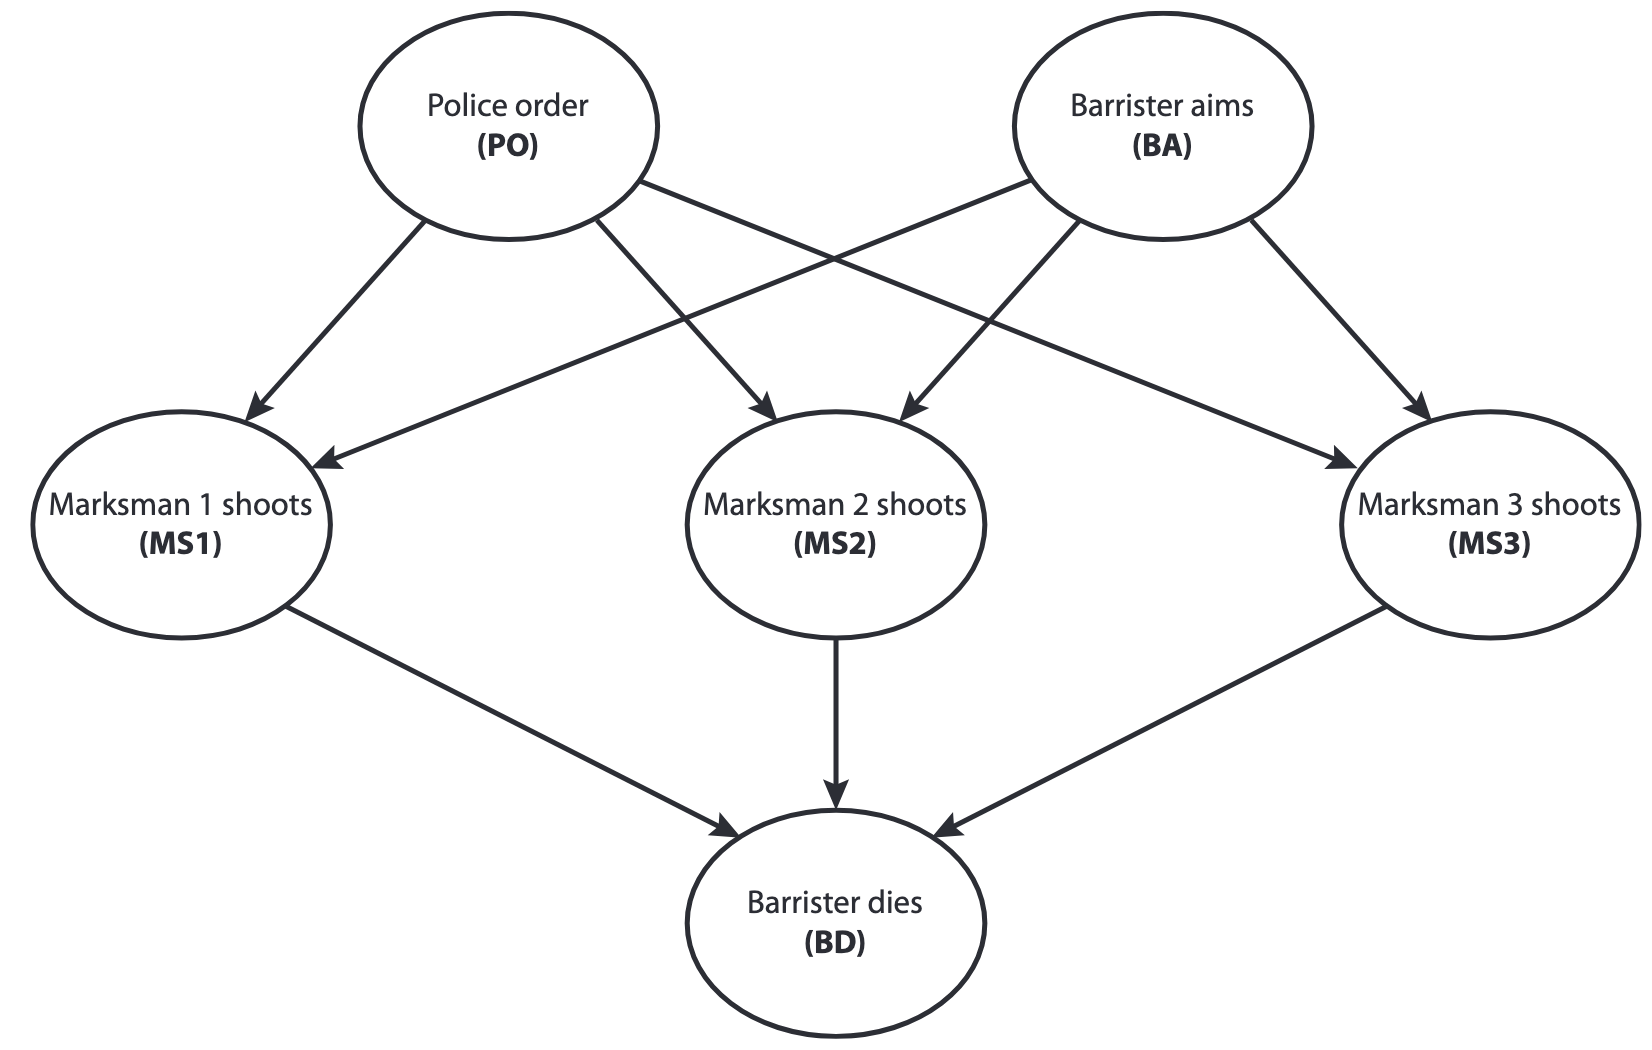
\includegraphics[width=.35\textwidth]{graphs/bn3}
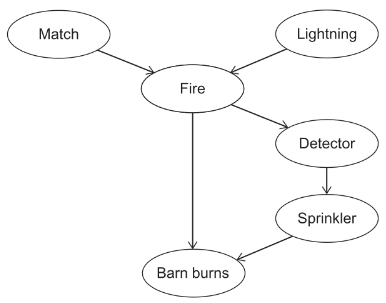
\includegraphics[width=.38\textwidth]{graphs/dag3}
\end{figure}

\par\begin{spacing}{.5}\begingroup\tiny (\href{https://doi.org/10.1111/cogs.12054}{Lagnado et al., 2014}; \href{https://www.cambridge.org/gb/universitypress/subjects/psychology/cognition/explaining-evidence-how-mind-investigates-world?format=PB}{Lagnado, 2021}; \href{https://doi.org/10.1146/annurev-psych-010814-015135}{Sloman \& Lagnado, 2015}; \href{https://doi.org/10.1007/s11229-025-04969-w}{Pilditch et al., 2025}).\endgroup\end{spacing}

\end{frame}

%
\begin{frame}{\color{darkblue}Building blocks for causal models}

\begin{columns}
\begin{column}{.05\textwidth}
\end{column}
\begin{column}{0.1\textwidth}
\centering
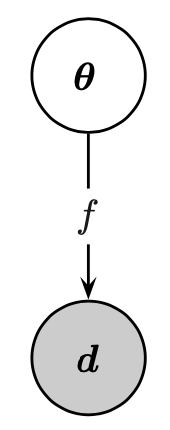
\includegraphics[width = .5\textwidth]{graphs/m1}\\
\tiny{Not hierarchical}
\end{column}
\begin{column}{0.1\textwidth}
\centering
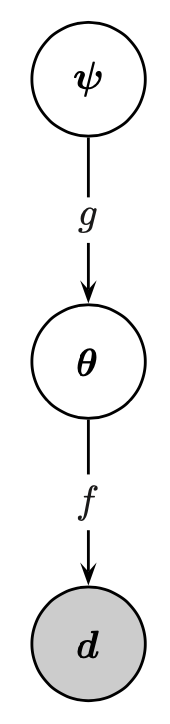
\includegraphics[width = .5\textwidth]{graphs/m2}\\
\tiny{Chain}
\end{column}
\begin{column}{0.2\textwidth}
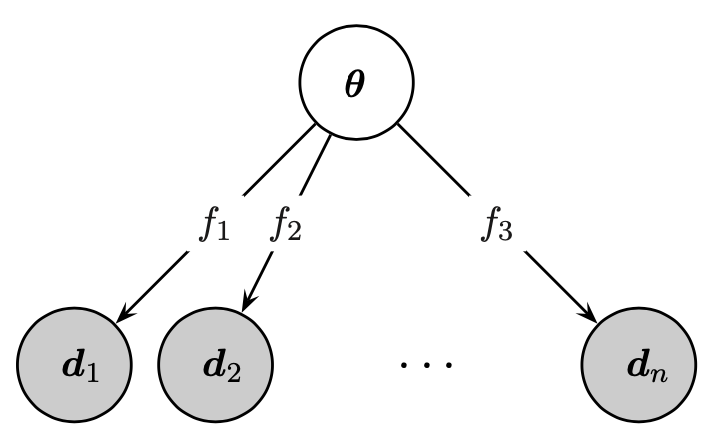
\includegraphics[width = 1\textwidth]{graphs/m3}\\
\centering
\tiny{Common-cause}
\end{column}
\begin{column}{0.2\textwidth}
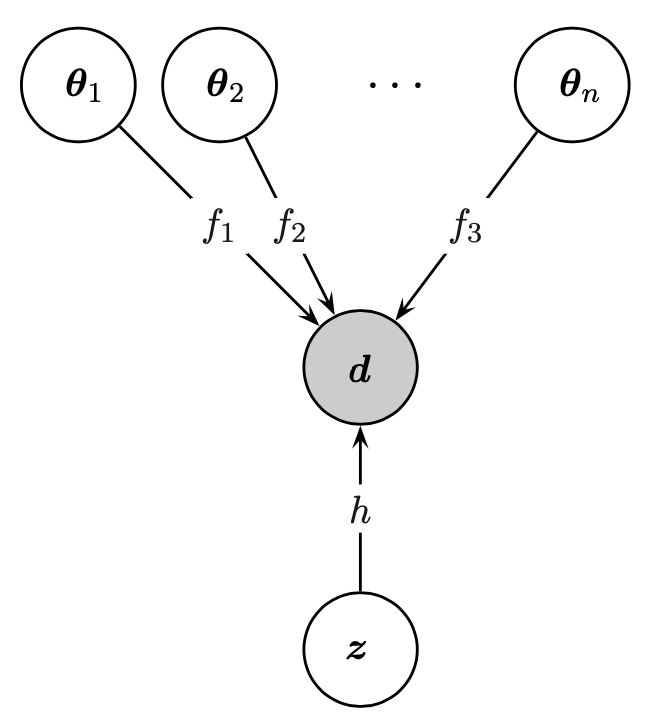
\includegraphics[width = 1\textwidth]{graphs/m4}\\
\centering
\tiny{Common-effect}
\end{column}
\begin{column}{0.2\textwidth}
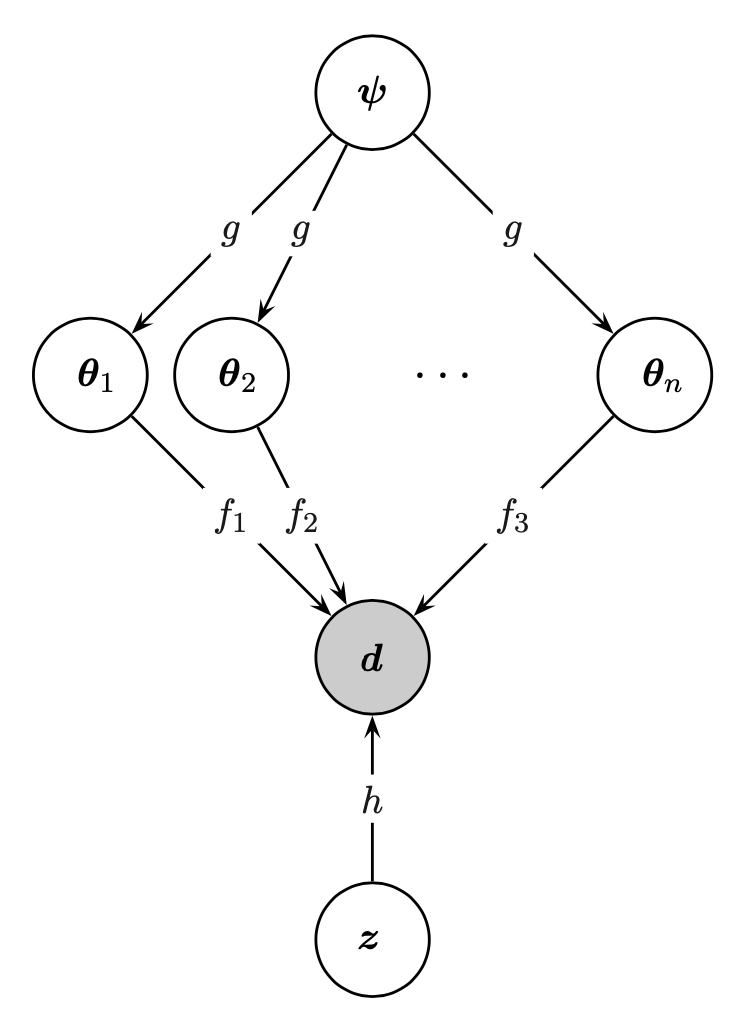
\includegraphics[width = 1\textwidth]{graphs/m5}\\
\centering
\tiny{Komplexer}
\end{column}
\begin{column}{0.05\textwidth}
\end{column}
\end{columns}


\par\begin{spacing}{.5}\begingroup\tiny (\href{https://doi.org/10.1016/j.jmp.2010.08.013}{Lee, 2011}).\endgroup\end{spacing}

\end{frame}

%
\begin{frame}{\color{darkblue}Binomial models}

\begin{columns}
\begin{column}{0.09\textwidth}
\end{column}
\begin{column}{0.5\textwidth}
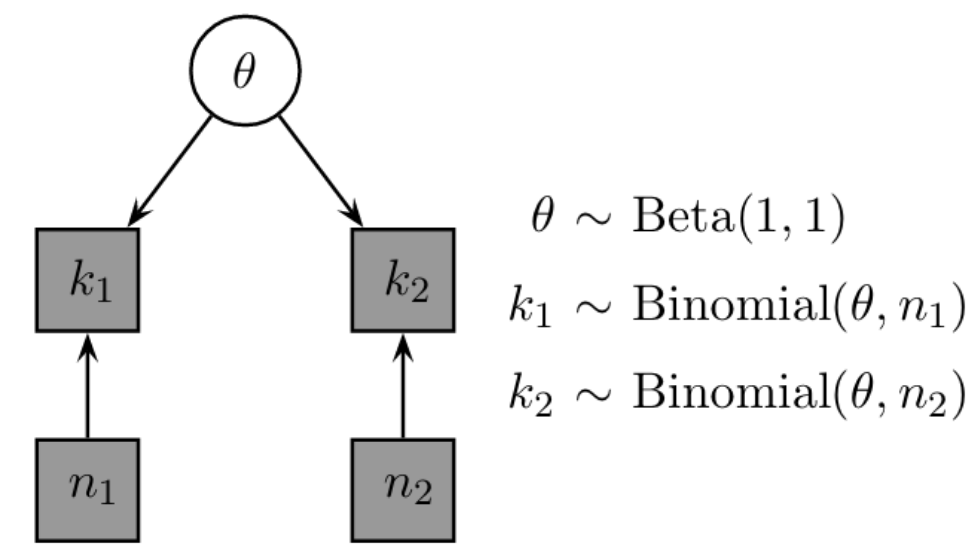
\includegraphics[width = .92\textwidth]{graphs/m6b} \\
\tiny{$\theta$ = Common probability \\that two coins land on heads}
\end{column}
\begin{column}{0.5\textwidth}
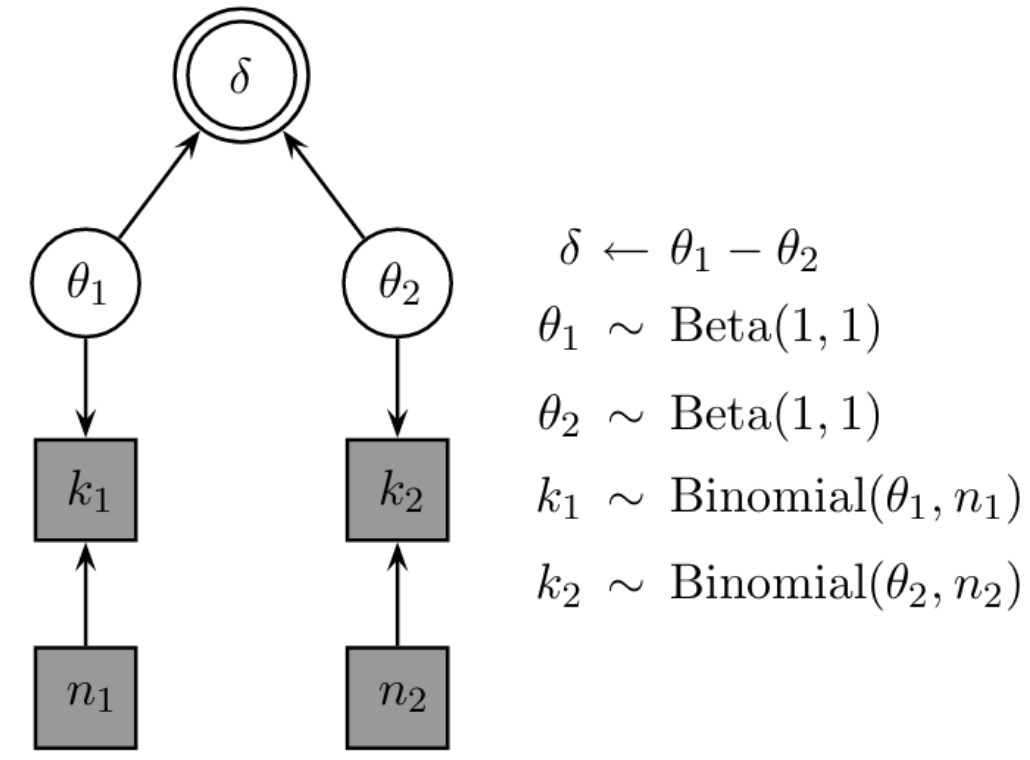
\includegraphics[width = .92\textwidth]{graphs/m7b} \\
\tiny{$\delta$ = Difference between \\ two probabilities}
\end{column}
\begin{column}{0.01\textwidth}
\end{column}
\end{columns}
\vspace{.3cm}

\pause
\begin{itemize}
\tightlist
\item {\color{teal}{squared}}: discrete vs. {\color{teal}{round}}: continuous
\item {\color{teal}{shaded}}: observed vs. {\color{teal}{unshaded}}: latent
\item {\color{teal}{double border}}: variable value is fully determined by the values of the variables that link to it. 
\end{itemize}

\par\begin{spacing}{.5}\begingroup\tiny (\href{https://doi.org/10.1017/CBO9781139087759}{Lee \& Wagenmakers, 2013}).\endgroup\end{spacing}

\end{frame}


%
\begin{frame}{\color{darkblue}Random-walk models}

\begin{columns}
\begin{column}{.5\textwidth}
\centering
\footnotesize{\color{teal}{Drift diffusion (DDM)}}
\end{column}
\begin{column}{.5\textwidth}
\centering
\footnotesize{\color{teal}{Linear ballistic accumulator (LBA)}}
\end{column}
\end{columns}

\begin{figure}
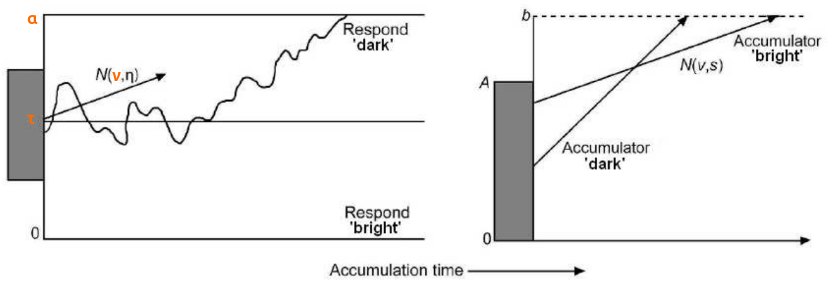
\includegraphics[width = .9\textwidth]{graphs/randomwalk2}
\end{figure}
\hfill
\pause

\begin{columns}[c]
\begin{column}{.10 \textwidth}
\end{column}
\begin{column}{.45 \textwidth}
\begin{center}
\small{\color{bluegray}{Latent DDM variables}}
\end{center}
\small{
\begin{itemize}
\tightlist
\item[-] drift rate \textbf{{\color{darkorange}{$\nu$}}}
\item[-] boundary separation \textbf{{\color{darkorange}{$\alpha$}}}
\item[-] nondecision time \textbf{{\color{darkorange}{$\tau$}}}
\end{itemize}
}
\end{column}

\begin{column}{.1\textwidth}
\centering

\hspace{-1cm}
\vspace{-1cm}
\begin{huge}
\color{bluegray}{
$\Longleftrightarrow$
}
\end{huge}
\end{column}

\begin{column}{.45 \textwidth}
\begin{center}
\small{\color{bluegray}{Observed variables}}
\end{center}
\small{
\begin{itemize}
\tightlist
\item[-] accuracy rate
\item[-] mean of correct RTs
\item[-] variance of correct RTs
\end{itemize}
}
\end{column}
\begin{column}{.1 \textwidth}
\end{column}
\end{columns}

\par\begin{spacing}{.5}\begingroup\tiny(\href{https://doi.org/10.1016/j.cogpsych.2007.12.002}{Brown \& Heathcote, 2008}; \href{https://doi.org/10.3758/s13423-025-02729-y}{Chávez De la Peña \& Vandekerckhove, 2025}; \href{https://www.researchgate.net/publication/277816660_Is_the_Linear_Ballistic_Accumulator_Model_Really_the_Simplest_Model_of_Choice_Response_Times_A_Bayesian_Model_Complexity_Analysis}{Donkin et al., 2009}).\endgroup\end{spacing}


\end{frame}

\end{document}